% !TeX program = pdflatex
\documentclass[tikz,border=8pt]{standalone}
\usepackage{tikz}\usetikzlibrary{angles,quotes,calc}
\definecolor{FigureBlue}{HTML}{2563EB}\definecolor{FigureOrange}{HTML}{EA580C}
\begin{document}
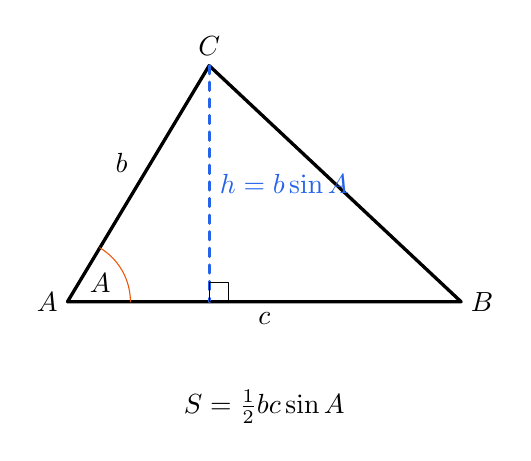
\begin{tikzpicture}[line cap=round,line join=round]
  \coordinate (A) at (0,0); \coordinate (B) at (5,0); \coordinate (C) at (1.8,3); \coordinate (D) at (1.8,0);
  \draw[line width=1.2pt] (A)--node[below] {$c$}(B)--(C)--node[above left] {$b$}(A);
  \draw[FigureBlue,dashed,line width=1.1pt] (C)--(D) node[midway,right] {$h=b\sin A$};
  \draw (D) rectangle ++(.25,.25); \pic[draw=FigureOrange,angle radius=8mm,"$A$"] {angle=B--A--C};
  \node[left] at (A) {$A$}; \node[right] at (B) {$B$}; \node[above] at (C) {$C$};
  \node[below=10mm] at ($(A)!.5!(B)$) {$S=\frac12bc\sin A$};
\end{tikzpicture}
\end{document}
